\documentclass[twoside,11pt]{article}

% Any additional packages needed should be included after jmlr2e.
% Note that jmlr2e.sty includes epsfig, amssymb, natbib and graphicx,
% and defines many common macros, such as 'proof' and 'example'.
%
% It also sets the bibliographystyle to plainnat; for more information on
% natbib citation styles, see the natbib documentation, a copy of which
% is archived at http://www.jmlr.org/format/natbib.pdf

\usepackage{csc498project}
\usepackage{url}
\usepackage{graphicx}
\graphicspath{ {./images/} }
\usepackage{float}


% Short headings should be running head and authors last names

\ShortHeadings{Atari Breakout Reinforcement Learning Environment}{Your names}
\firstpageno{1}


\title{Atari Breakout Reinforcement Learning Environment}

\author{\name Haider Sajjad \email haider.sajjad@mail.utoronto.ca \\
       \addr 1004076251\\
       \AND
      \name Weiyu Li \email weiyu.li@mail.utoronto.ca \\
       \addr 1003765981}

\begin{document}

\maketitle

\begin{abstract}%   <- trailing '%' for backward compatibility of .sty file
\textit{
Atari Breakout environment implementation and training an agent using multiple algorithms over a generated environment (changing brick layouts)}

\end{abstract}

\section{Introduction}
Our project is implementing an Atari breakout environment and training an agent to play it across general levels. The project repository can be found here: \url{https://github.com/duoduocai-dot/csc498-project} To play the original game, after cloning the project, just run this file: \url{https://github.com/duoduocai-dot/csc498-project/blob/main/run_Breakout.py}.\\
Our environment is \href{https://github.com/duoduocai-dot/csc498-project/blob/main/breakout.py}{here}. We made a made our environment embedded into a pygame class for Breakout, adding environment functions and variables. \\
We made 6 algorithms which play Breakout, and compare their performance in this report. The algorithms we made are: DQN, double-DQN, policy gradient REINFORCE, tabular Q-Learning, tabular double Q-Learning, and tabular SARSA.

\section{Environment}
Our environment is here: \url{https://github.com/duoduocai-dot/csc498-project/blob/main/breakout.py}.
\subsection{Rewards}
We experimented with various reward mechanisms. Our original reward schema was:
\begin{itemize}
\item +10 for ball hitting paddle
\item -10 ball missing paddle
\item +1 ball hits brick
\item -0.2 movement penalty
\item +1000 ball destroys all bricks
\end{itemize}
However, with this model we noticed it was difficult for the agent to actually learn, as it doesn't get direct feedback if making an action is good or not. So we altered the reward schema to be:
\begin{itemize}
\item +10 for ball hitting paddle
\item -10 ball missing paddle
\item Distance between paddle and ball in the x-Axis \url{https://github.com/duoduocai-dot/csc498-project/blob/main/breakout.py#L179}
\item +1000 ball destroys all bricks
\end{itemize}
\subsection{Environment variables, functions} 
Regarding the rest of the environment, the step function is \href{https://github.com/duoduocai-dot/csc498-project/blob/f46268a6c9241b77efd6c96a6dd8ecc3ec5bae1e/breakout.py#L266}{here}, where the paddle moves depending on the action passed in, and updates rewards for that step. It then returns the game state which is \href{https://github.com/duoduocai-dot/csc498-project/blob/f46268a6c9241b77efd6c96a6dd8ecc3ec5bae1e/breakout.py#L246}{[paddle x-location, ball x-location, ball y-location,ball x-speed, ball y-speed, bricks left]}.
\\
The \href{https://github.com/duoduocai-dot/csc498-project/blob/f46268a6c9241b77efd6c96a6dd8ecc3ec5bae1e/breakout.py#L299}{reset} function resets the environment, setting ball, bricks, paddle to their original position. 
\\ \href{https://github.com/duoduocai-dot/csc498-project/blob/f46268a6c9241b77efd6c96a6dd8ecc3ec5bae1e/breakout.py#L316}{Render} functio, renders the game. \href{https://github.com/duoduocai-dot/csc498-project/blob/f46268a6c9241b77efd6c96a6dd8ecc3ec5bae1e/breakout.py#L332}{Make} function creates the brick layout, and \href{https://github.com/duoduocai-dot/csc498-project/blob/f46268a6c9241b77efd6c96a6dd8ecc3ec5bae1e/breakout.py#L335}{main function} allows the user to play the game. 
\\
Agent actions are to \href{https://github.com/duoduocai-dot/csc498-project/blob/f46268a6c9241b77efd6c96a6dd8ecc3ec5bae1e/breakout.py#L270}{move left (0), move right (1), stay still (2)}.
\\
There is more about the environment including the \href{https://github.com/duoduocai-dot/csc498-project/blob/f46268a6c9241b77efd6c96a6dd8ecc3ec5bae1e/breakout.py#L55}{brickLayout} which we used in testing and comparing the tabular algorithms which I will talk about in that section.  

\section{Algorithims}

\subsection{Tabular Algorithms}
We made 3 algorithms which utilize a tabular setup. We reduced the state sizes such that they could be discretized, and fit inside a table.
\\\\
How we created the tabular setup is by first getting every possible paddle and ball locations
using this \href{https://github.com/duoduocai-dot/csc498-project/blob/main/tabular_Q_learning.py#L223}{discretizeStateSpaceAllStates function} which splits the paddle x-locations into 20 possible locations, the ball x-locations into 80 possible locations, and ball y-locations into 30 possible locations. The game screen is 800x600 and paddle is 80 wide and ball is 5x5.
\\\\
I experimented with 3 different schemas to discretize the state space. These included:
\begin{itemize}
\item \href{https://github.com/duoduocai-dot/csc498-project/blob/main/tabular_Q_learning.py#L180}{10 paddle locations, 40 ball x-locations, 20 ball y-locations}
\item \href{https://github.com/duoduocai-dot/csc498-project/blob/main/tabular_Q_learning.py#L203}{10 paddle locations, 80 ball x-locations, 30 ball y-locations}
\item \href{https://github.com/duoduocai-dot/csc498-project/blob/main/tabular_Q_learning.py#L223}{20 paddle locations, 80 ball x-locations, 30 ball y-locations}
\end{itemize}
The last one with the most paddle and ball locations worked best:\\\\\\
\begin{figure}[h]
Here are the rewards from the last 10 episodes of training using the fewest number of states (first bullet):\\
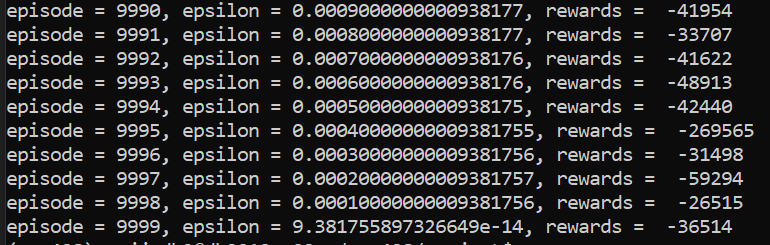
\includegraphics[scale=0.5]{rewards_last_10_episodes_fewest_number_states}
\centering
\end{figure}
\begin{figure}[h]
Compared the rewards from the last 10 episodes of training using the most states (last bullet):\\
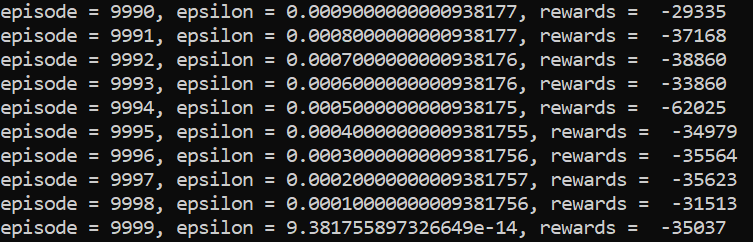
\includegraphics[scale=0.5]{rewards_last_10_episodes_largest_number_states}
\centering
\\ It's clear that the larger number of states gives more rewards.
\end{figure}
\\\\\\
After, we (\url{https://github.com/duoduocai-dot/csc498-project/blob/main/tabular_Q_learning.py#L37}) just create a dictionary to store the policy and Q-values, with every possible state using the schema above.

\subsubsection{\href{https://github.com/duoduocai-dot/csc498-project/blob/main/tabular_Q_learning.py}{Tabular Q-Learning}}
For tabular Q-Learning, now with a table of all possible states, we can just apply the Q-Learning epsilon greedy algorithm. Where the Q-Learning step:
\begin{equation}
Q(s_t,a_t) \leftarrow Q(s_t,a_t) + \alpha (r_t + \gamma max_a Q(s_{t+1},a) - Q(s_t,a_t))
\end{equation}

This exact Q-Learning update can be found \href{https://github.com/duoduocai-dot/csc498-project/blob/main/tabular_Q_learning.py#L88}{here}. Where we get the Q-value at each action for the next state, and plug in the max Q-value for the next state into the equation.
\\\\
The other important aspect of Q-Learning is the epsilon-greedy exploration. We first initialize our \href{https://github.com/duoduocai-dot/csc498-project/blob/main/tabular_Q_learning.py#L54}{epsilon in the class}, then it is updated after every \href{https://github.com/duoduocai-dot/csc498-project/blob/main/tabular_Q_learning.py#L285}{episode}. The policy is updated for every state inside the \href{https://github.com/duoduocai-dot/csc498-project/blob/main/tabular_Q_learning.py#L103}{q\_learning function} using the same epsilon-greedy approach. 
\\
For the epsilon decay, to increase exploitation rather than exploration, instead of the usual $\epsilon = \epsilon/k$ approach, \href{https://github.com/duoduocai-dot/csc498-project/blob/main/tabular_Q_learning.py#L285}{we used a $\epsilon = \epsilon + decay$ where decay} is usually some negative number between 0 and 1.

\subsubsection{\href{https://github.com/duoduocai-dot/csc498-project/blob/main/tabular_double_Q_learning.py}{Tabular Double Q-Learning}}
In tabular double Q-Learning, our \href{https://github.com/duoduocai-dot/csc498-project/blob/main/tabular_double_Q_learning.py}{algorithm} is nearly the exact same as tabular Q-Learning, except we maintain \href{https://github.com/duoduocai-dot/csc498-project/blob/main/tabular_double_Q_learning.py#L40}{two} Q-value dictionaries and each one is updated with 0.5 \href{https://github.com/duoduocai-dot/csc498-project/blob/main/tabular_double_Q_learning.py#L91}{probability}.
Pseudocode for double Q-Learning:
\\
Select $a_t$ using epsilon greedy $\pi(s) = argmax_a Q_1(s_t, a)+Q_2(s_t, a)$ 
\\
with 0.5 probability:

\begin{equation}
Q_1(s_t,a_t) \leftarrow Q_1(s_t,a_t) + \alpha (r_t + \gamma Q_1(s_{t+1}, argmax_a Q_2(s_{t+1},a)) - Q_1(s_t,a_t))
\end{equation}
else:
\begin{equation}
Q_2(s_t,a_t) \leftarrow Q_2(s_t,a_t) + \alpha (r_t + \gamma Q_2(s_{t+1}, argmax_a Q_1(s_{t+1},a)) - Q_2(s_t,a_t))
\end{equation}

\subsubsection{\href{https://github.com/duoduocai-dot/csc498-project/blob/main/Sarsa.py}{Tabular Sarsa}}
Tabular SARSA, implementation is similar to the above two, discretization of state space and epsilon-greedy exploration are both implemented the same way. Except the Q-value update is done using a \href{https://github.com/duoduocai-dot/csc498-project/blob/main/Sarsa.py#L80}{bootstrapped one-step look ahead}, like in the algorithm:
\begin{equation}
Q(s_t,a_t) \leftarrow Q(s_t,a_t) + \alpha (r_t + \gamma Q(s_{t+1},a_{t+1}) - Q(s_t,a_t))
\end{equation}

\subsubsection{Training} 
To train each of the algorithms, there is a training function which creates an instance of the algorithm then loops through a number of episodes collecting states, actions and rewards and using them for training. The code to run the training is commented out at the end of each file for \href{https://github.com/duoduocai-dot/csc498-project/blob/main/Sarsa.py#L281}{SARSA}, \href{https://github.com/duoduocai-dot/csc498-project/blob/main/tabular_Q_learning.py#L307}{QL}, and \href{https://github.com/duoduocai-dot/csc498-project/blob/main/tabular_double_Q_learning.py#L326}{Double-QL}

\subsection{Comparing tabular algorithms} 
{
Here is a direct comparison of all 3 algorithms trained over 10000 episodes for 5000 steps per. It's clear from the pictures that Q-Learning and double Q-Learning outpreform SARSA.
\begin{figure}[H]
Rewards Comparison of all 3 tabular algorithms and the last 3000 episodes comparison:\\
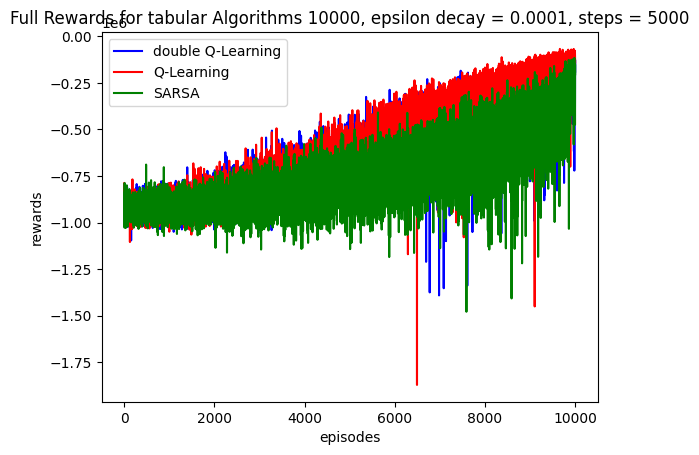
\includegraphics[scale=0.4]{Full_Rewards_Comparison1}
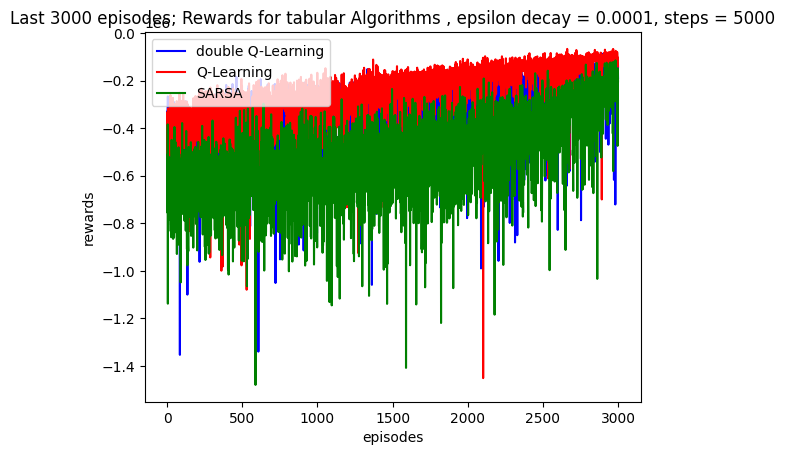
\includegraphics[scale=0.4]{Last_3000_rewards_comparison1}
\centering
\end{figure}
}
\subsubsection{Performance}
All 3 tabular algorithms do achieve good performance and are able to play the game effectively.
\\
Here are graphs for all 3 algorithms, it's clear that as episodes increase and epsilon grows smaller, all 3 algorithms achieve higher rewards. These graphs were made \\
----pictures----
\subsubsection{Parameter and Hyperparameter Choice}
In the tabular algorithms there were many parameters that we used: epsilon and decay-value, episodes, stepsize, learning rate ($\alpha$),  discount ($\gamma$).
\\\\
The choice of epsilon was simply just 1. We wanted lots of exploration in the beginning, for the agent to learn the environment. The epsilon decay was implemented such that: $\epsilon = \epsilon + decay$. The reason for this is because we wanted a linear decrease of epsilon to account for lots of exploration
\subsubsection{Q-Learning maximization problems}
\subsubsection{Generalized tests}
\subsubsection{Which Layout is best to train on?}
Talk about
\begin{itemize}
\item epsilon choice and decay choice, step and episode size
\item preformance of each algorithm
\item maximization problem with Q-Learning, and how altering reward schema can fix it.
\item How the above can be fixed with a different epsilon greedy approach (epsilon goes down to 0, then up to 1, then back down, repeats for n times, when it ends its at 0). This approach is to make sure there is enough exploration in the later regions of the game.
\item comparing algorithms in generalized tests, also talk about generalized brick layouts
\item Talk about which bricklayout is best to train on to maximize most generalization of agent (bricklayout1)
\end{itemize}

\subsection{Policy Gradient}
talk about
\begin{itemize}
\item problems with original reward schema and how because of policy gradient we altered it
\item gradients getting trapped in local mins/maxes
\item fixes for this which can include lowering learning rate, using momentum in gradient or using soft-actor-critic, or using exploration
\item talk about the epsilon-greedy exploration currently implemented
\end{itemize}


\bibliography{bibliography}

\end{document}